\subsection{Idee}\label{ss:Idee}

Nicht nur für Museen, Villen oder Betriebe ist ein Sicherheitssystem sinnvoll, denn besonders in private Wohnungen und Häuser wird gerne eingebrochen.

\begin{figure}[H] 
	\centering
	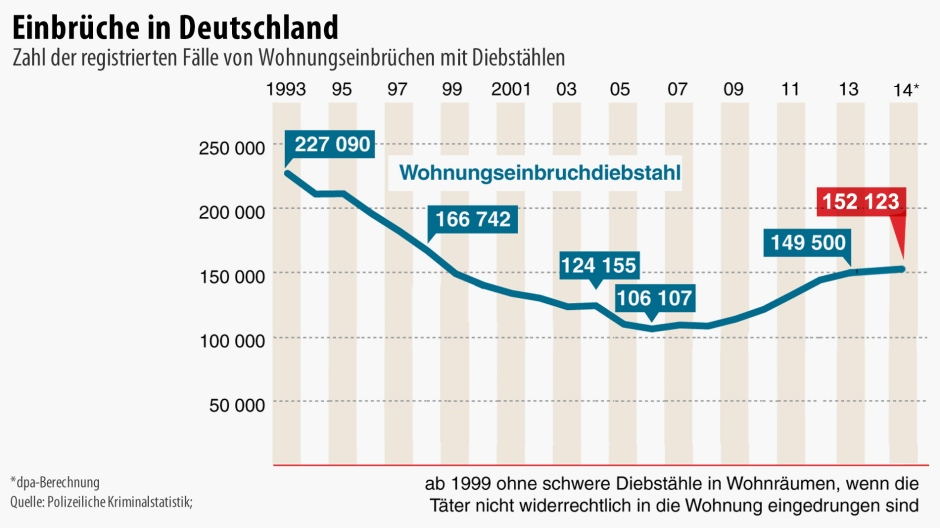
\includegraphics[scale=0.35]{Bilder/einbrueche}
	\caption{Einbruchsstatistik in Deutschland\cite{i:einbrueche}}
	\label{f:einrbrueche}
\end{figure}

Allein im Jahr 2014 wurde über 150.000 mal in Deutschland ein Einbruch mit Diebstahl gemeldet. Die Aufklärungsrate der Verbrechen hingegen ist jedoch sehr gering. Um sich vor solchen Straftaten zu schützen werden Überwachungsanlagen immer beliebter.\\
Im Rahmen dieser Studienarbeit soll eine Raumüberwachung entwickelt werden, die mit Hilfe von untereinander vernetzten Sensoren Einbrüche frühzeitig erkennt, und an den Besitzer meldet. Die Überwachung soll direkt an Fenster und Türen stattfinden, mit Hilfe von Vibrationssensoren, Mikrophonen oder Kameras sollen außergewöhnliche Vorkommnisse ausgewertet werden. Bei einem Einbruch kann dies dem Besitzer über das Netzwerk mitgeteilt werden.

